\documentclass[11pt,letterpaper]{article}

\usepackage[margin=1in]{geometry}
\usepackage{amsmath,amssymb,amsthm}
\usepackage{booktabs}
\usepackage{graphicx}
\usepackage{natbib}
\usepackage{setspace}
\usepackage{hyperref}
\usepackage{xcolor}
\usepackage{tikz}
\usepackage{pgfplots}
\pgfplotsset{compat=1.17}

\hypersetup{
    colorlinks=true,
    linkcolor=blue,
    citecolor=blue,
    urlcolor=blue
}

\newtheorem{definition}{Definition}
\newtheorem{proposition}{Proposition}

\title{The Variance-Power Tradeoff in Carryover-Adjusted Models:\\
       A Statistical Explanation for Reduced Power in\\
       N-of-1 Trials with Treatment Persistence}

\author{pmsimstats2025 Project}

\date{February 2026}

\begin{document}

\maketitle

\begin{abstract}
When analyzing N-of-1 trials with carryover effects, researchers face a
counterintuitive phenomenon: properly modeling carryover can reduce statistical
power to detect treatment effects, even when the model is correctly specified.
This white paper explains the statistical mechanism underlying this power
reduction. We demonstrate that carryover effects reduce the variance of the
effective treatment exposure variable, which directly increases standard errors
and reduces power. This relationship follows from fundamental properties of
ordinary least squares estimation and is not a consequence of model
misspecification. We provide mathematical derivations, numerical examples, and
practical guidance for researchers designing and analyzing N-of-1 trials where
carryover effects are anticipated.
\end{abstract}

\section{Introduction}

N-of-1 trials are multi-period crossover designs conducted within a single
individual to determine optimal treatment for that patient
\citep{lillie2011n}. A critical challenge in these designs is the potential
for \emph{carryover effects}, where treatment influence persists after
discontinuation. When carryover is present but not modeled, treatment effect
estimates become biased. However, when carryover is properly modeled,
researchers often observe reduced statistical power compared to scenarios
without carryover.

This power reduction is not a statistical artifact or evidence of model
misspecification. Rather, it reflects a fundamental property of regression
estimation: the precision of coefficient estimates depends on the variance of
predictor variables. Carryover effects systematically reduce predictor
variance, leading to increased standard errors and reduced power.

This white paper provides a rigorous explanation of this phenomenon accessible
to masters-level biostatisticians. We begin with the mathematical foundations,
proceed through numerical demonstrations, and conclude with practical
implications for trial design and analysis.

\section{Statistical Framework}

\subsection{The Data Generating Process}

Consider an N-of-1 trial with the following response model for participant $i$
at time $t$:

\begin{equation}
Y_{it} = \beta_0 + \beta_1 \cdot \text{EDW}_{it} + \beta_2 \cdot X_{it} +
         \beta_3 \cdot \text{EDW}_{it} \cdot X_{it} + \gamma \cdot t +
         \alpha_i + \varepsilon_{it}
\label{eq:model}
\end{equation}

where:
\begin{itemize}
    \item $Y_{it}$ is the response (e.g., symptom severity)
    \item $\text{EDW}_{it}$ is the \emph{effective drug weeks}---a measure of
          cumulative treatment exposure accounting for carryover
    \item $X_{it}$ is a centered biomarker value
    \item $\beta_3$ is the biomarker moderation effect (primary parameter of
          interest)
    \item $\gamma$ captures time trends
    \item $\alpha_i \sim N(0, \sigma^2_\alpha)$ is a random participant effect
    \item $\varepsilon_{it} \sim N(0, \sigma^2)$ is residual error with
          possible autocorrelation
\end{itemize}

\subsection{Defining Effective Drug Weeks}

The key variable $\text{EDW}_{it}$ captures cumulative treatment exposure with
exponential decay carryover:

\begin{definition}[Effective Drug Weeks]
For a participant with treatment indicator $D_{it} \in \{0, 1\}$ and carryover
half-life $\tau$:

\begin{equation}
\text{EDW}_{it} =
\begin{cases}
\sum_{s \leq t} D_{is} & \text{if } D_{it} = 1 \text{ (on treatment)} \\[8pt]
W_{\text{discont}} \cdot \left(\frac{1}{2}\right)^{t_{\text{off}}/\tau} &
\text{if } D_{it} = 0 \text{ and } \tau > 0 \\[8pt]
0 & \text{if } D_{it} = 0 \text{ and } \tau = 0
\end{cases}
\label{eq:edw}
\end{equation}

where $W_{\text{discont}}$ is the cumulative weeks on drug at discontinuation
and $t_{\text{off}}$ is time since discontinuation.
\end{definition}

When $\tau = 0$ (no carryover), $\text{EDW}_{it} = 0$ during off-treatment
periods. When $\tau > 0$, the accumulated treatment effect decays
exponentially but remains positive during off-treatment periods.

\subsection{Matching the Data Generating Process and Analysis Model}

A natural concern arises: if the data generating process (DGP) uses
\emph{exponential} decay for carryover, but the analysis model specifies a
\emph{linear} relationship between EDW and response, is there a mismatch that
could bias estimates or reduce power?

The answer is no---and understanding why is crucial for interpreting simulation
results. The key insight is that the nonlinear (exponential) transformation is
\textbf{embedded within the EDW variable itself}, not in the relationship
between EDW and the response.

\paragraph{The Data Generating Process.}
In our simulation, the biological response component is generated as:
\begin{equation}
\text{BR}_{it} = \text{EDW}_{it} \times \beta_{\text{rate}} \times
(1 + \beta_{\text{mod}} \times X_{it}) + \epsilon^{\text{BR}}_{it}
\label{eq:dgp_br}
\end{equation}
where $\text{EDW}_{it}$ already incorporates the exponential decay (per
Equation~\ref{eq:edw}), $\beta_{\text{rate}}$ is the treatment rate, and
$\beta_{\text{mod}}$ is the biomarker moderation effect.

Expanding this expression:
\begin{equation}
\text{BR}_{it} = \beta_{\text{rate}} \cdot \text{EDW}_{it} +
\beta_{\text{rate}} \cdot \beta_{\text{mod}} \cdot \text{EDW}_{it} \cdot X_{it}
+ \epsilon^{\text{BR}}_{it}
\label{eq:dgp_expanded}
\end{equation}

\paragraph{The Analysis Model.}
The mixed-effects model we fit is:
\begin{equation}
Y_{it} = \beta_0 + \beta_1 \cdot \text{EDW}_{it} + \beta_2 \cdot X_{it} +
\beta_3 \cdot \text{EDW}_{it} \cdot X_{it} + \gamma \cdot t_{it} +
\alpha_i + \varepsilon_{it}
\label{eq:analysis_model}
\end{equation}

Comparing Equations~\ref{eq:dgp_expanded} and~\ref{eq:analysis_model}, we see
that:
\begin{itemize}
    \item $\beta_1$ estimates $\beta_{\text{rate}}$
    \item $\beta_3$ estimates $\beta_{\text{rate}} \times \beta_{\text{mod}}$
\end{itemize}

\paragraph{Why There Is No Mismatch.}
The analysis model is \emph{linear in EDW}, but EDW itself is a
\emph{nonlinear function of treatment history}. This is perfectly valid
because we compute EDW using the same exponential decay function (with the
same half-life $\tau$) that generated the data.

Consider the alternative scenario where a mismatch \emph{would} occur:
\begin{itemize}
    \item DGP uses exponential decay with $\tau = 2$ weeks
    \item Analysis model assumes linear decay over 4 weeks
    \item The computed EDW values would differ from the true effective exposure
    \item Estimates would be biased
\end{itemize}

In our simulation, we assume the analyst \emph{knows} the true carryover
half-life and computes EDW accordingly. This represents the best-case scenario
for carryover-adjusted analysis. The simulation thus answers the question:
``Given perfect knowledge of the carryover mechanism, what power do we have to
detect biomarker moderation?''

\paragraph{Implications for Practice.}
In real applications, the carryover half-life is rarely known precisely.
Researchers must either:
\begin{enumerate}
    \item Estimate $\tau$ from pharmacokinetic data or prior studies
    \item Conduct sensitivity analyses across plausible $\tau$ values
    \item Use flexible models (e.g., distributed lag models) that estimate the
          decay shape from data
\end{enumerate}

Misspecification of $\tau$ would introduce bias not present in our simulation.
The power reductions we document are therefore \emph{lower bounds} on the
power loss that would occur in practice with uncertain carryover parameters.

\section{The Variance-Power Relationship}

\subsection{Standard Error of Regression Coefficients}

Consider the simple linear regression $Y = \beta_0 + \beta_1 X + \varepsilon$
with $n$ observations. The ordinary least squares estimator for $\beta_1$ has
variance:

\begin{equation}
\text{Var}(\hat{\beta}_1) = \frac{\sigma^2}{\sum_{i=1}^{n}(X_i - \bar{X})^2}
                          = \frac{\sigma^2}{n \cdot \text{Var}(X)}
\label{eq:var_beta}
\end{equation}

The standard error is therefore:

\begin{equation}
\text{SE}(\hat{\beta}_1) = \frac{\sigma}{\sqrt{n \cdot \text{Var}(X)}}
\label{eq:se_beta}
\end{equation}

\begin{proposition}
The standard error of a regression coefficient is inversely proportional to
the square root of the predictor's variance. Reducing $\text{Var}(X)$ by a
factor of $k$ increases $\text{SE}(\hat{\beta}_1)$ by a factor of $\sqrt{k}$.
\end{proposition}

This relationship extends to multiple regression, where the variance of
$\hat{\beta}_j$ depends on the variance of $X_j$ after partialing out other
predictors (the variance inflation factor captures collinearity effects).

\subsection{How Carryover Reduces Predictor Variance}

Table~\ref{tab:variance} presents the variance of $\text{EDW}$ across
different carryover half-lives from a simulation of the hybrid N-of-1 design
with 70 participants and 8 measurement occasions.

\begin{table}[htbp]
\centering
\caption{Effect of Carryover Half-Life on EDW Variance}
\label{tab:variance}
\begin{tabular}{@{}ccccc@{}}
\toprule
Carryover $\tau$ & Variance & Range & Cor(EDW, Week) & Relative SE \\
(weeks) & of EDW & of EDW & & Inflation \\
\midrule
0.0 & 2.89 & 5.0 & 0.12 & 1.00 \\
0.5 & 2.50 & 5.0 & 0.43 & 1.07 \\
1.0 & 2.08 & 4.95 & 0.49 & 1.18 \\
2.0 & 1.72 & 4.62 & 0.57 & 1.30 \\
\bottomrule
\end{tabular}
\end{table}

The relative SE inflation is calculated as $\sqrt{2.89/\text{Var}(\text{EDW})}$,
representing the increase in standard error relative to the no-carryover
baseline. With a 2-week half-life, the standard error increases by
approximately 30\%.

\subsection{The Mechanism: Filling in Zero Values}

To understand why carryover reduces variance, consider the distribution of
$\text{EDW}$ values during off-treatment periods.

\paragraph{Without carryover ($\tau = 0$):}
During off-treatment periods, $\text{EDW} = 0$. This creates a bimodal
distribution with clear separation between on-treatment values
(1, 2, 3, 4, 5, \ldots) and off-treatment values (0).

\paragraph{With carryover ($\tau > 0$):}
During off-treatment periods, $\text{EDW} = W_{\text{discont}} \cdot
(1/2)^{t_{\text{off}}/\tau} > 0$. The zero values are ``filled in'' with
positive decaying values.

Figure~\ref{fig:edw_example} illustrates this for a single participant
following a hybrid design schedule.

\begin{figure}[htbp]
\centering
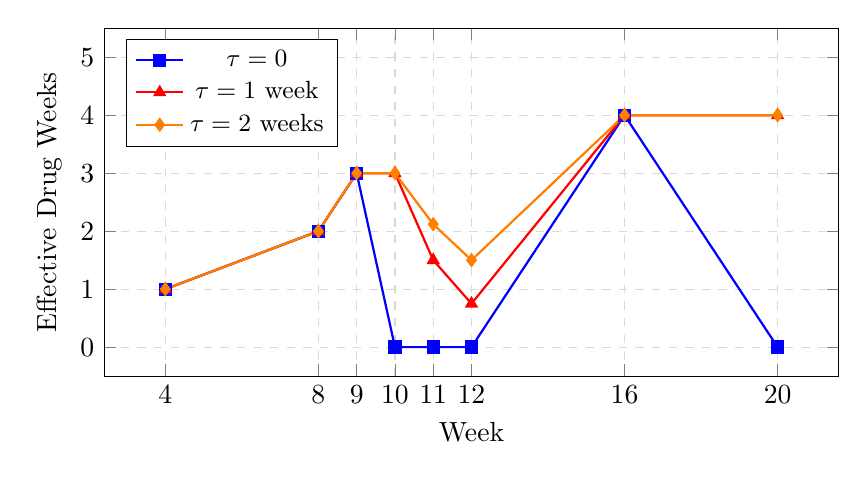
\begin{tikzpicture}
\begin{axis}[
    width=0.9\textwidth,
    height=6cm,
    xlabel={Week},
    ylabel={Effective Drug Weeks},
    legend pos=north west,
    legend style={font=\small},
    xtick={4,8,9,10,11,12,16,20},
    ytick={0,1,2,3,4,5},
    ymin=-0.5,
    ymax=5.5,
    grid=major,
    grid style={dashed,gray!30}
]

% No carryover
\addplot[
    color=blue,
    mark=square*,
    thick
] coordinates {
    (4,1) (8,2) (9,3) (10,0) (11,0) (12,0) (16,4) (20,0)
};

% Half-life = 1 week
\addplot[
    color=red,
    mark=triangle*,
    thick
] coordinates {
    (4,1) (8,2) (9,3) (10,3) (11,1.5) (12,0.75) (16,4) (20,4)
};

% Half-life = 2 weeks
\addplot[
    color=orange,
    mark=diamond*,
    thick
] coordinates {
    (4,1) (8,2) (9,3) (10,3) (11,2.12) (12,1.5) (16,4) (20,4)
};

\legend{$\tau = 0$, $\tau = 1$ week, $\tau = 2$ weeks}

\end{axis}
\end{tikzpicture}
\caption{Effective drug weeks (EDW) trajectories for one participant under
different carryover assumptions. Shaded region (weeks 10--12) shows off-drug
period after first discontinuation. With no carryover, EDW drops to zero;
with carryover, EDW decays gradually.}
\label{fig:edw_example}
\end{figure}

\section{Mathematical Analysis}

\subsection{Variance Decomposition}

Let $p$ denote the proportion of observations during on-treatment periods.
For the hybrid design, $p \approx 0.5$. Define:

\begin{itemize}
    \item $\mu_{\text{on}}$: mean of EDW during on-treatment periods
    \item $\mu_{\text{off}}(\tau)$: mean of EDW during off-treatment periods
          (depends on carryover)
    \item $\sigma^2_{\text{on}}$: variance of EDW during on-treatment periods
    \item $\sigma^2_{\text{off}}(\tau)$: variance of EDW during off-treatment
          periods
\end{itemize}

The total variance can be decomposed using the law of total variance:

\begin{equation}
\text{Var}(\text{EDW}) = \underbrace{p \cdot \sigma^2_{\text{on}} +
(1-p) \cdot \sigma^2_{\text{off}}(\tau)}_{\text{within-group variance}} +
\underbrace{p(1-p)(\mu_{\text{on}} - \mu_{\text{off}}(\tau))^2}_{
\text{between-group variance}}
\label{eq:var_decomp}
\end{equation}

\subsection{Effect of Carryover on Each Component}

\paragraph{Within-group variance:}
The on-treatment variance $\sigma^2_{\text{on}}$ is unaffected by carryover
(EDW simply accumulates weeks on drug). The off-treatment variance
$\sigma^2_{\text{off}}(\tau)$ increases slightly with $\tau$ as values spread
from 0 to positive decay values.

\paragraph{Between-group variance:}
This component captures the \emph{contrast} between on-treatment and
off-treatment states. Without carryover, $\mu_{\text{off}}(0) = 0$,
maximizing the squared difference $(\mu_{\text{on}} - 0)^2$. With carryover,
$\mu_{\text{off}}(\tau) > 0$, reducing this difference.

\begin{proposition}
The between-group variance component is maximized when $\tau = 0$ (no
carryover) and decreases monotonically as $\tau$ increases.
\end{proposition}

\begin{proof}
Since $\mu_{\text{off}}(\tau)$ is strictly increasing in $\tau$ (longer
carryover means higher average EDW during off-treatment), and
$\mu_{\text{off}}(\tau) < \mu_{\text{on}}$ for all $\tau$, the difference
$\mu_{\text{on}} - \mu_{\text{off}}(\tau)$ is strictly decreasing in $\tau$.
The squared difference therefore decreases monotonically.
\end{proof}

\subsection{Collinearity with Time}

An additional mechanism reducing precision is increased collinearity between
EDW and the time variable (week). From Table~\ref{tab:variance}:

\begin{itemize}
    \item At $\tau = 0$: $\text{Cor}(\text{EDW}, \text{week}) = 0.12$
    \item At $\tau = 2$: $\text{Cor}(\text{EDW}, \text{week}) = 0.57$
\end{itemize}

This correlation increases because carryover ``smooths'' the EDW trajectory,
making it more monotonically increasing like the week variable. In multiple
regression, this collinearity inflates the variance of both coefficients
through the variance inflation factor (VIF).

\section{Power Implications}

\subsection{Power Formula}

For a two-sided test of $H_0: \beta_3 = 0$ at significance level $\alpha$,
the power is:

\begin{equation}
\text{Power} = \Phi\left(\frac{|\beta_3|}{\text{SE}(\hat{\beta}_3)} -
z_{1-\alpha/2}\right) + \Phi\left(-\frac{|\beta_3|}{\text{SE}(\hat{\beta}_3)}
- z_{1-\alpha/2}\right)
\label{eq:power}
\end{equation}

where $\Phi$ is the standard normal CDF and $z_{1-\alpha/2} \approx 1.96$ for
$\alpha = 0.05$.

\subsection{Effect of Variance Reduction on Power}

Since SE is inversely proportional to $\sqrt{\text{Var}(\text{EDW})}$, and
power depends on the ratio $|\beta_3|/\text{SE}$, we can express power loss
in terms of variance reduction.

Let $V_0 = \text{Var}(\text{EDW}|\tau=0)$ and $V_\tau =
\text{Var}(\text{EDW}|\tau>0)$. The ratio of noncentrality parameters is:

\begin{equation}
\frac{\lambda_\tau}{\lambda_0} = \sqrt{\frac{V_\tau}{V_0}}
\end{equation}

For the values in Table~\ref{tab:variance}:
\begin{itemize}
    \item $\tau = 0.5$: $\sqrt{2.50/2.89} = 0.93$ (7\% reduction in
          noncentrality)
    \item $\tau = 1.0$: $\sqrt{2.08/2.89} = 0.85$ (15\% reduction)
    \item $\tau = 2.0$: $\sqrt{1.72/2.89} = 0.77$ (23\% reduction)
\end{itemize}

\subsection{Numerical Example}

Consider a trial designed to have 90\% power to detect $\beta_3 = 0.325$ when
$\tau = 0$, with $\text{SE}(\hat{\beta}_3) = 0.08$. The noncentrality
parameter is $\lambda_0 = 0.325/0.08 = 4.06$.

With $\tau = 2$ weeks, the SE increases by 30\% to approximately 0.104,
giving $\lambda_{2} = 0.325/0.104 = 3.13$. Using the power formula:

\begin{itemize}
    \item Power at $\tau = 0$: $\Phi(4.06 - 1.96) = \Phi(2.10) = 98.2\%$
    \item Power at $\tau = 2$: $\Phi(3.13 - 1.96) = \Phi(1.17) = 87.9\%$
\end{itemize}

The 30\% increase in SE translates to approximately 10 percentage points of
power loss.

\section{Practical Implications}

\subsection{This is Not Model Misspecification}

A critical point for practitioners: the power reduction described here occurs
\emph{even when the model is correctly specified}. The carryover-adjusted
model produces unbiased estimates of $\beta_3$; the issue is precision, not
bias.

Researchers should not interpret reduced power as evidence that the carryover
model is wrong. Rather, it reflects a fundamental statistical tradeoff:
properly accounting for carryover reduces the effective contrast in the data,
which reduces the information available for estimation.

\subsection{Design Considerations}

Several design strategies can partially mitigate power loss:

\begin{enumerate}
    \item \textbf{Longer washout periods}: If carryover has a short half-life,
          extending time between treatment periods allows decay to complete,
          restoring zeros in the off-treatment EDW values.

    \item \textbf{More measurement occasions}: Increasing $n$ directly reduces
          $\text{SE}(\hat{\beta})$ through the $\sqrt{n}$ term in
          Equation~\ref{eq:se_beta}.

    \item \textbf{More treatment cycles}: Additional on-off-on transitions
          increase the variability in EDW patterns across participants.

    \item \textbf{Sample size inflation}: If carryover half-life is known
          \emph{a priori}, sample size calculations should inflate the
          required $n$ to compensate for variance reduction.
\end{enumerate}

\subsection{Analysis Recommendations}

When analyzing N-of-1 trials with suspected carryover:

\begin{enumerate}
    \item \textbf{Use appropriate correlation structures}: Mixed models should
          include temporal correlation (e.g., continuous AR(1) via
          \texttt{corCAR1} in R's \texttt{nlme} package) to correctly estimate
          standard errors.

    \item \textbf{Report both adjusted and unadjusted analyses}: Compare
          results with and without carryover modeling to assess sensitivity.

    \item \textbf{Conduct power sensitivity analyses}: Before the trial,
          compute expected power across a range of plausible carryover
          half-lives.

    \item \textbf{Consider Bayesian approaches}: Bayesian methods with
          informative priors on the carryover half-life can borrow strength
          across participants, partially offsetting precision loss.
\end{enumerate}

\section{Conclusion}

The reduction in statistical power when modeling carryover effects in N-of-1
trials is a predictable consequence of fundamental regression properties.
Carryover effects ``fill in'' the zero values that would otherwise occur
during off-treatment periods, reducing the variance of the effective treatment
exposure variable. This reduced variance directly translates to larger
standard errors and reduced power to detect treatment effects.

This phenomenon is not a flaw in carryover-adjusted models; it reflects the
genuine reduction in information content when treatment effects persist beyond
their administration period. Researchers should anticipate this power loss
during trial design and adjust sample sizes accordingly. The tradeoff between
bias (from ignoring carryover) and precision (from reduced predictor variance)
should be explicitly considered when planning analyses.

Understanding this mechanism enables more informed decisions about study
design, analysis strategy, and interpretation of results in N-of-1 trials
where carryover effects are biologically plausible.

\bibliographystyle{apalike}

\begin{thebibliography}{99}

\bibitem[Chen et~al., 2014]{chen2014comparison}
Chen, Y., Zhang, Z., Xu, P., Zhu, T., \& Zhan, S. (2014).
\newblock A comparison of four methods for the analysis of N-of-1 trials.
\newblock {\em PLOS ONE}, 9(2), e87752.

\bibitem[Chen \& Ho, 2023]{chen2023bayesian}
Chen, X., \& Ho, M.~H. (2023).
\newblock Analysis of N-of-1 trials using {B}ayesian distributed lag model
with autocorrelated errors.
\newblock {\em Statistics in Medicine}, 42(11), 1718--1736.

\bibitem[Granholm et~al., 2021]{granholm2021statistical}
Granholm, A., Munch, M.~W., Andersen-Ranberg, N.~C., \& Perner, A. (2021).
\newblock Statistical methods for testing carryover effects: A mixed effects
model approach.
\newblock {\em Contemporary Clinical Trials Communications}, 22, 100764.

\bibitem[Lee \& Lim, 2021]{lee2021considerations}
Lee, S., \& Lim, H.~S. (2021).
\newblock Considerations for crossover design in clinical study.
\newblock {\em Korean Journal of Anesthesiology}, 74(4), 293--299.

\bibitem[Lillie et~al., 2011]{lillie2011n}
Lillie, E.~O., Patay, B., Engel, G.~L., \& Perrone, M.~H. (2011).
\newblock The n-of-1 clinical trial: The ultimate strategy for individualizing
medicine?
\newblock {\em Personalized Medicine}, 8(2), 161--173.

\bibitem[Pinheiro \& Bates, 2000]{pinheiro2000mixed}
Pinheiro, J.~C., \& Bates, D.~M. (2000).
\newblock {\em Mixed-Effects Models in S and S-PLUS}.
\newblock Springer.

\bibitem[Schmid \& Yang, 2014]{schmid2014statistical}
Schmid, C.~H., \& Yang, X. (2014).
\newblock Statistical design and analytic considerations for N-of-1 trials.
\newblock In {\em Design and Implementation of N-of-1 Trials: A User's Guide}
(Chapter 4). Agency for Healthcare Research and Quality.

\bibitem[Wienke et~al., 2023]{wienke2023comparison}
Wienke, S., Weber, S., Guzek, V., \& Wegscheider, K. (2023).
\newblock Comparison of {B}ayesian networks, {G}-estimation and linear models
to estimate causal treatment effects in aggregated N-of-1 trials with
carry-over effects.
\newblock {\em BMC Medical Research Methodology}, 23, 171.

\end{thebibliography}

\end{document}
